%%%%%%%%%%%%%%%%%%%%%%%%%%%%%%%%%%%%%%%%%%%%%%%%%%%%%%%
% Please note that whilst this template provides a 
% preview of the typeset manuscript for submission, it 
% will not necessarily be the final publication layout.
%
% letterpaper/a4paper: US/UK paper size toggle
% num-refs/alpha-refs: numeric/author-year citation and bibliography toggle

%\documentclass[letterpaper]{oup-contemporary}
\documentclass[a4paper,num-refs]{oup-contemporary}

%%% Journal toggle; only specific options recognised.
%%% (Only "gigascience" and "general" are implemented now. Support for other journals is planned.)
\journal{analog}

%\usepackage{fontspec}
%\setmainfont[Mapping=tex-text]{KaiTi}

\usepackage{graphicx}
\graphicspath{{Pics/}{logo/}}
\usepackage{subfigure}
\usepackage{siunitx}
\usepackage{amssymb}
\usepackage{hyperref}
\usepackage{stfloats}

%% Flushend: You can add this package to automatically balance the final page, but if things go awry (e.g. section contents appearing out-of-order or entire blocks or paragraphs are coloured), remove it!
% \usepackage{flushend}

\title{Super Capacitor and Its Digital Controller for Robotic Power Management}

%%% Use the \authfn to add symbols for additional footnotes, if any. 1 is reserved for correspondence emails; then continuing with 2 etc for contributions.
\author[1,\authfn{1}]{Hongyi Zhou}
\author[2,\authfn{1}]{Wuzizheng Zhong}
\author[2,\authfn{1}]{Yutong Wei}
\author[2,\authfn{1}]{Zhou Chen}

\affil[1]{Optoelectronic Engineering}
\affil[2]{Cybernetics Engineering}

%%% Author Notes
\authnote{\authfn{1}12110322@mail.sustech.edu.cn; 12112613@mail.sustech.edu.cn; 12112549@mail.sustech.edu.cn; 12111812@mail.sustech.edu.cn}



%%% Paper category
\papercat{Project Report}

%%% "Short" author for running page header
\runningauthor{Edited by CooperChou}

%%% Should only be set by an editor
\jvolume{01}
\jnumber{1}
\jyear{2022}

\begin{document}

\begin{frontmatter}
\maketitle
\begin{abstract}
Limitation of power-batteries sometimes restricted the performance of robots, with insufficient instantaneous power supply and finite energy. Before the advancement of solid state batteries, methods of instantaneous power compensation are worth priority for diminishing robot sizes as well as increasing power efficiency. In this work, based on the compensation demand, we focus on the design of a super capacitor module controlled by a digital DC-DC bidirectional rectifier, which aims at the optimization of robotic battery energy. We have already managed the hardware-design and basic functional trials of the rectifier and super capacitor, which is now able to regulate the power of the module according to a given number. However, the stability, efficiency, ripple and response time remains to be optimized.
\end{abstract}

\begin{keywords}
Power compensation; super capacitor; rectifier; optimization; power management
\end{keywords}
\end{frontmatter}


\begin{epigraph}{Albert Einstein}
Science is a wonderful thing if one does not have to earn one's living at it.
\end{epigraph}


\section{I. Introduction}

\subsection{Background}

Along with the progress of technology in the $ 21_{st} $ century, the application of mobile robots is widened and simplified, resulting in various robotic products in either civil and industrial vision. However, the application might reach a choke-neck at a certain coming time when present battery is not able to meet the demand of some scenarios, such as robots requiring both small size and large output torque or high motion speed which ask for small\footnote{Both in mass and dimension.} battery but also large output power or current. Before the birth of advanced solid state batteries or other types of high-performance battery, the development of corresponding robots might be blocked. 

In addition, the power management of robot is also a crucial part in raising power efficiency, which means to have energy appropriately distributed, stored and spent, either energy from the power source or the recyclable loss\footnote{For example, if possible, the thermal energy produced everywhere on a robot, or the back electromotive force when braking. In fact, $ Tesla^{\circledR} $ has already done a great job on the latter one.}.

From the problems and demands stated above, it came to our mind that a module with energy absorption and releasing function, a.k.a. the ability to store energy may be suitable for the scenario. Therefore, we determined our target on such a device.

\subsection{Application Scenario}

\subsubsection{Requirements}
As mentioned, the device can not be a general battery, because the demand calls for devices bearing large power or current with small size. The first idea was capacitors or inductors for their energy storing nature, but the latter were then abandoned for their bulky size. So the decision eventually came down on building a super capacitor.

Apart from the size and power restriction, precise and fast response are equally significant for a robotic system, so a digital regulator takes similar priority.

Accordingly, our corresponding refined tasks were:
\begin{itemize}
	\item A super capacitor group with sufficient energy capacity and current endurance
	\item A digital regulator and its software program with the capability to absorb and release power according to given amounts as fast as possible
\end{itemize}

\subsubsection{Scenario Assumption}
For task-simplification, we set our oriented scenario to be a mobile robot system with characteristics below:

\begin{table}[h]
	\begin{center}
		\begin{tabular}{r l}
			\textbf{Supply Voltage} & $ 24V $ \\
			\hline
			\textbf{Source Power Limit} & $ 120W $ \\
			\hline
			\textbf{Maximum Required Power}& $ 200W $ \\
		\end{tabular}
	\end{center}
\end{table} 

And the topology of our module in a robot system is supposed to be:
\begin{figure}[h]
	\centering
	\includegraphics[width=0.5\linewidth]{ChassisTopology.png}
	\caption{Topology of the Module in a Robotic System}
\end{figure} 
%**************************************************

\section{II. Project Process}
\subsection{Demand Analysis}
According to the itemized tasks, refined scheme and design were made as follows:

\subsubsection{Super Capacitor Module}
Based on comprehensive consideration, the sufficient energy capacity of the capacitor module lies at about 2000J; the extra power requirement of 80W calls for an extra current of about 3.33A under 24V, which requires a current endurance of at least 4A for stability; the bulky sizes of single capacitors with large capacitance are not worth effort compared to groups of smaller capacitors.

So we decided to combine 9 super capacitors with 60F capacitance and 2.7V maximum voltage in series, yielding 1920J at 24V\footnote{For safety, we would not charge it to 24.3V($ 9*2.7V = 24.3V $).}, and the capacitor we selected to use is produced by $ Cda^{\circledR} $\footnote{Official website of $ Cda^{\circledR} $: \href{http://www.cda-cap.com/}{http://www.cda-cap.com/}}, and owns an endurance current of 4.58A, which is qualified.

Nevertheless, the tiny difference between capacitors may result in damage as uneven energy distribution happens, a.k.a. some capacitors may be overcharged while others are not fully charged. So we search and found a specified chip called BW6101 from $ BITWELL^{\circledR} $\footnote{Official website of $ BITWELL^{\circledR} $: \href{http://www.bitwell.com.cn/}{http://www.bitwell.com.cn/}}, aiming directly in protecting super capacitor from overcharge. But the discharge current of 1A seems not sufficient for our module, thus a transistor is added to enlarge the current, as well as to low resistance resistor with package R2512 for thermal dissipation.

\begin{figure}[h]
	\centering
	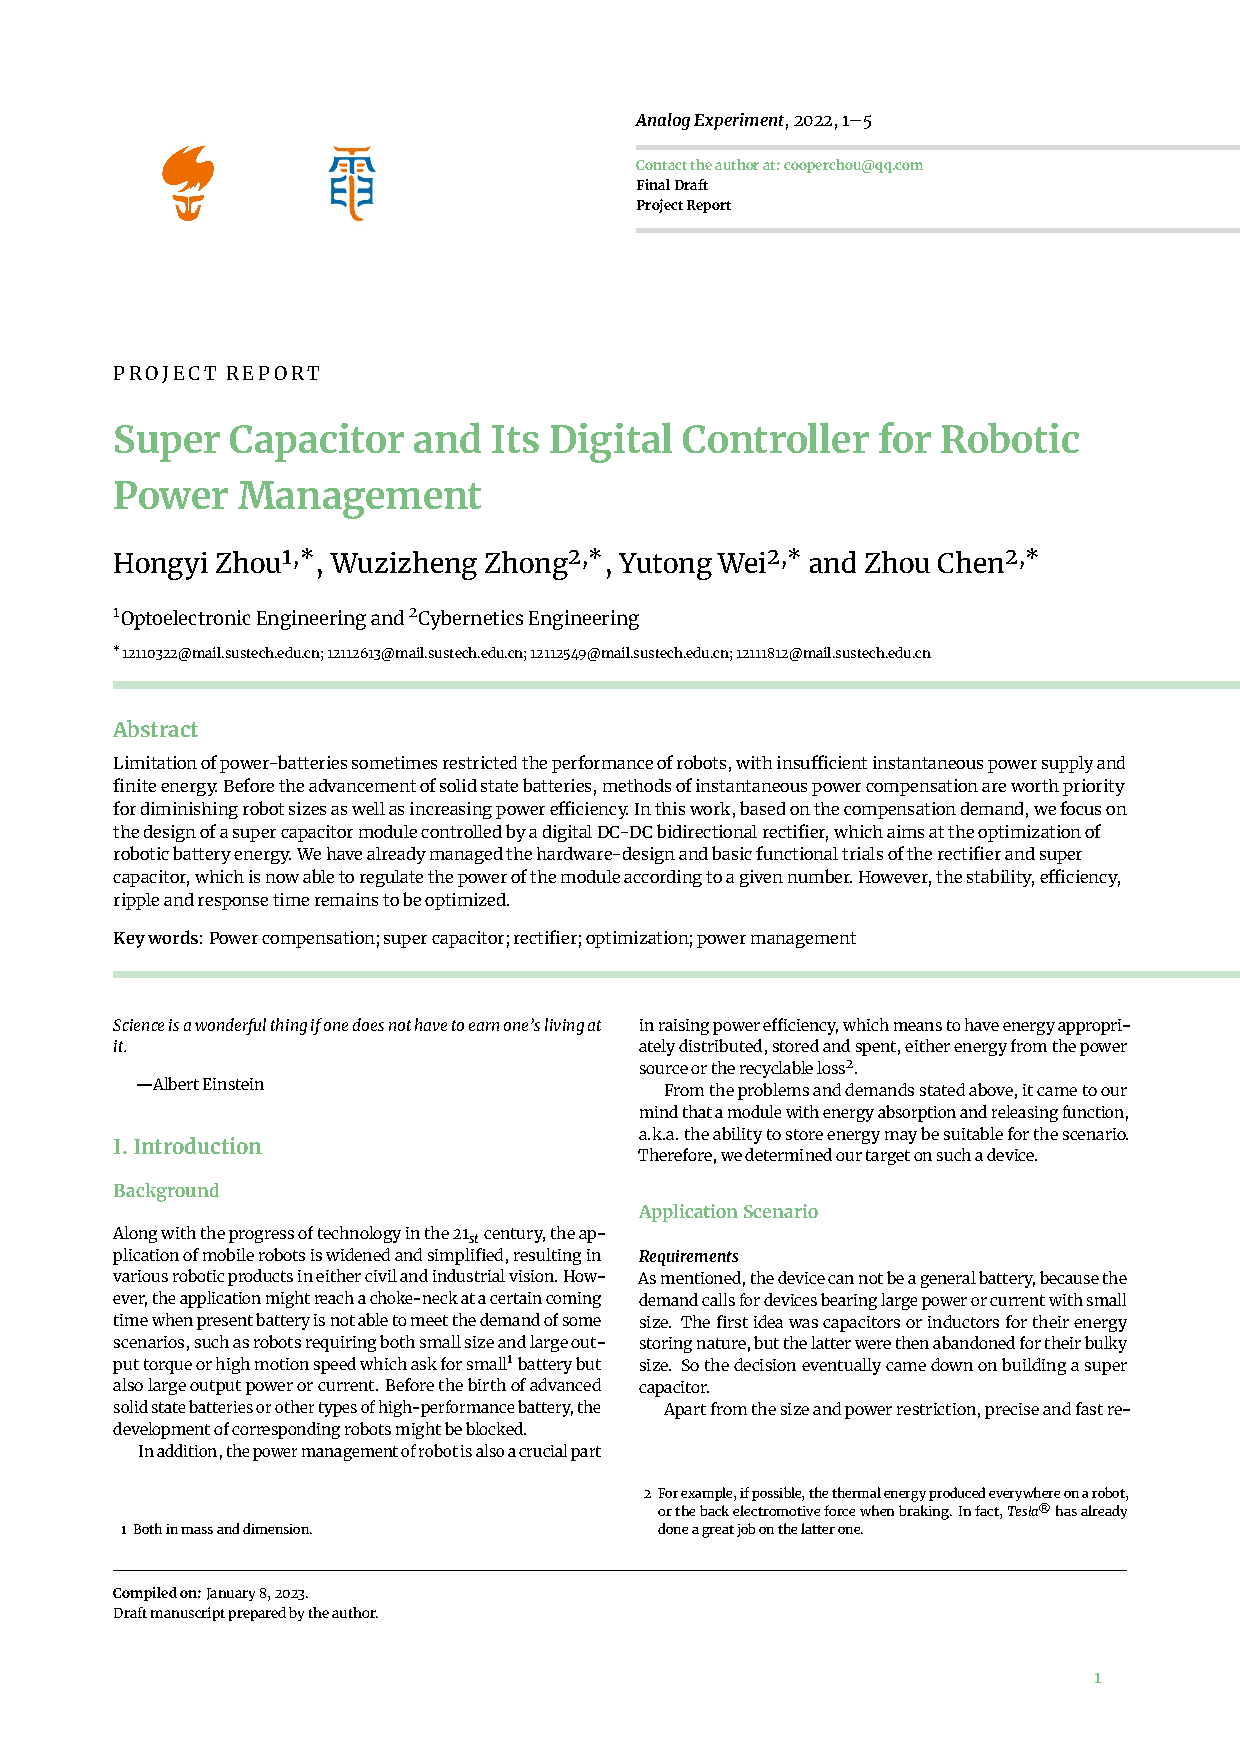
\includegraphics[width=0.8\linewidth]{SuperCapacitor.png}
	\caption{One of the Nine Capacitors and Their Peripheral Circuits}
\end{figure} 

\subsubsection{Regulator}
The aim of precisely controlling the charging and discharging power requires DC-DC voltage modification as well as bidirectional power flow; to consume the capacitor energy as completely as possible, BUCK function must be involved; to charge the capacitor with sufficient current when its voltage is approaching 24V, the designed fully charged voltage of the capacitor module, BOOST function is also needed.

The only two structure we Knew were Synchronous SEPIC rectifier and Bidirectional Synchronous BUCK-BOOST rectifier. The latter one is eventually chosen for the complex regulation program of the former.

\begin{figure}[h]
	\centering
	\includegraphics[width=0.8\linewidth]{BuckBoost.png}
	\caption{The Bidirectional Synchronous BUCK-BOOST Structure}
\end{figure} 

The most crucial elements in the circuit are the MOSFETs, which are the most frequently damaged parts. After comparison and research, BSC070N10NS3G from $ Infineon^{\circledR} $\footnote{Official website of $ Infineon^{\circledR} $: \href{https://www.infineon.com/cms/en/}{https://www.infineon.com/cms/en/}} was selected, for its adequate parameters and relatively low price(About 10RMB each). 


\begin{table}[h]
	\begin{center}
		\begin{tabular}{r l}
			$ V_{DS} $ & $ 100V $ \\
			\hline
			$ R_{DS(on),max} $ & $ 7m\Omega $ \\
			\hline
			$ I_D $ & $ 90A $ \\
		\end{tabular}
	\end{center}
\end{table} 

However, simple MOSFET selection is insufficient for a well-performing switching rectifier, and proper driver and Layout is required. So we chose two UCC27211's from $ Texas Instrument^{\circledR} $\footnote{Official website of $ Texas Instrument^{\circledR} $: \href{https://www.ti.com/}{https://www.ti.com/}} for H-bridge driving, and applied STM32F334C8T6 from $ STMicroelectronics^{\circledR} $\footnote{Official website of $ STMicroelectronics^{\circledR} $: \href{https://www.st.com/content/st_com/en.html}{https://www.st.com/content/st\_com/en.html}} to drive the MOSFET driver, because MOSFETs in switching rectifiers are working under high-speed switching state with $ V_{GS} $ varying in a large range(About $ 0V~9.5V $ in this application) which a general MCU fails to offer. 

\begin{figure}[h]
	\centering
	\includegraphics[width=0.6\linewidth]{GateDriver.png}
	\caption{The Half-bridge Gate Driver}
\end{figure} 

In addition, to precisely control the behavior of the module, feedback takes high priority. The parameters required are the input and output voltages and currents of the regulator, so some sampling circuit are designed with utilization of the ADC feature of the MCU. Voltage sampling simply applies a bleeder circuit with impedance matching and filtering measures, while current sampling uses the difference amplifier INA240A1PWR from $ Texas Instrument^{\circledR} $ and a sampling resistor of $ 6m\Omega $ for its high common mode rejection ratio and PWM rejection ratio.

\begin{figure}[h]
	\centering
	\includegraphics[width=0.6\linewidth]{VoltageSampling.png}
	\caption{Voltage Sampling}
\end{figure} 

\begin{figure}[h]
	\centering
	\includegraphics[width=0.7\linewidth]{CurrentSampling.png}
	\caption{Current Sampling}
\end{figure} 


\subsubsection{Controlling Program}
There are three missions for the program:
\begin{itemize}
	\item Control the direction of power flow to charge or discharge the capacitor.
	\item Regulate the charging or discharging power precisely to satisfy actuators as well as make entire use of source power under the limit.
	\item Protect the module and the system from damage.
\end{itemize}
Proper realization of the missions would then be carried out through codes.

The strategy should be:
\begin{enumerate}
	\item The robot predict the power need in the next controlling period and then send it to the module.
	\item The module compute the extra power required by the actuator in accordance with the source power limit and received data.
	\item The module calculate the required current at the capacitor side according to the extra power, and thus yield the required voltage at the source side and the mapping PWM set.
	\item The module then judge whether the output\footnote{In fact, the output refers to the ratio electromotive force at the two sides of the regulator, which is decided by the PWM duty cycle that can be modified by the regulator}(related to the PWM set) will exceed the range of safety, and modulate it based on the range if necessary.
	\item Set the output of the module, and wait for the next period.
\end{enumerate}

When sampling electrical parameter through ADC, errors occur; and the relationship between PWM set and output is linear and thus predictable, so we found the fitting parameter through experiment.

\begin{figure}[h]
	\centering
	\includegraphics[width=0.8\linewidth]{PWMandVoltage.png}
	\caption{The Matching Between PWM Set and Output}
\end{figure} 

\begin{figure}[h]
	\centering
	\includegraphics[width=0.8\linewidth]{Multimeter.png}
	\caption{ADC Fitting}
\end{figure} 

In order to respond as soon as possible, the RC equation is applied for calculation, assisted with PID in calculation error compensation.
\begin{figure}[h]
	\centering
	\includegraphics[width=0.8\linewidth]{PIDandCal.png}
	\caption{Combination of Calculation and PID Feedback Control}
\end{figure} 


The module protection is also defined in the program.
\begin{figure}[h!]
	\centering
	\begin{minipage}[t]{0.8\linewidth}
		\centering
			\subfigure[Voltage limitation at the Capacitor Side]{
		\centering
		\includegraphics[width=0.8\linewidth]{Security.png}
	}
	\end{minipage}
\vfill
	\begin{minipage}[t]{0.8\linewidth}
		\centering
		\subfigure[Voltage limitation at the Actuator Side]{
		\centering
		\includegraphics[width=0.8\linewidth]{Security2.png}
	}
	\end{minipage}
\caption{Some of the Soft-Protections}
\end{figure} 

%**************************************************

\section{III. Outcome}
\subsection{Hardware Appearance}
The module hardware consists of three PCBs, which are, from top to bottom, Digital Controller, DC-DC Rectifier and Super Capacitor respectively. Also, a shell is designed and built through 3D printing for capacitor protection.
\begin{figure}[h]
	\centering
	\includegraphics[width=0.7\linewidth]{Look.jpg}
	\caption{Appearance of the Module}
\end{figure} 

\subsection{Functions}
\subsubsection{Bidirectional Power Flow Regulation}
Regulation of module power is realized, with an acceptable precision, as shown in Fig.\ref{Performance} .

\begin{figure*}[!bp]
		\centering
\begin{minipage}[t]{0.8\linewidth}
	\centering
	\subfigure[Regulator Quiescent Power Dissipation]{
		\begin{minipage}[t]{0.25\linewidth}
			\centering
			\includegraphics[height=\linewidth]{Off.jpg}
		\end{minipage}
	}
\hfill
	\subfigure[Zero Power Consumption Regulation]{
		\begin{minipage}[t]{0.25\linewidth}
			\centering
			\includegraphics[height=\linewidth]{Zero.jpg}
		\end{minipage}
}
\hfill
	\subfigure[Charging the Capacitor with 40W Module Power Consumption]{
	\begin{minipage}[t]{0.25\linewidth}
		\centering
		\includegraphics[height=\linewidth]{40WIn.jpg}
	\end{minipage}
}
\end{minipage}
\vfill
\begin{minipage}[t]{0.6\linewidth}
	\centering
\subfigure[Module in the System with Zero Energy Dissipation]{
	\begin{minipage}[t]{0.4\linewidth}
		\centering
		\includegraphics[height=\linewidth]{ZeroLoad.jpg}
	\end{minipage}
}
\hfill
\subfigure[Module in the System Providing 20W Extra Power]{
	\begin{minipage}[t]{0.4\linewidth}
		\centering
		\includegraphics[height=\linewidth]{20WLoad.jpg}
	\end{minipage}
}
	\centering
	\caption{Bidirectional Power Flow and Power Regulation(The digital power source is used to simulate the power source in a robotic system, while the electronic load above it simulating the actuator.)}
	\label{Performance}
\end{minipage}
\end{figure*}

\subsubsection{Module Power Regulation}
As shown in Fig.\ref{Performance}, the module managed to control the magnitude of power through itself. The precision has exceeded approximately 95\%, which is enough for a beginner.

\subsection{Characteristics}

\subsubsection{Efficiency of Regulator}
After calibration, the accuracy of ADC detected voltages and currents is sufficiently reliable, and according to the parameter shown in the \textit{Watch} of the \textit{Debug} interface of \textit{Keil} \footnote{Keil is a debugging software designed by $ Keil Software^{\circledR} $ from USA, aiming at development of Single Chip Microcomputer(or MCU) using C-Programming-Language.}, efficiency of the regulator is over 90\%.

\subsubsection{Ripple}
Rough measurements were done by simply contacting the probe stylus of oscilloscope with the regulator port, which resulted in detected ripples of 15.5mV under 40W module power and 11.6mV under 10W module power, as shown in Fig.\ref{ripple}.

However, after online searching, the tested ripples seem to be too small and beyond our standard, probably related to the unqualified testing environment. Therefore, the data owns low reliability.

\begin{figure}[h!]
	\centering
	\begin{minipage}{0.45\linewidth}
		\centering
		\subfigure[Ripple Waveform under 40W Module Power]{
		\centering
		\includegraphics[width = 0.8\linewidth]{40WRipple.png}
	}
	\end{minipage}
\hfill
	\begin{minipage}{0.45\linewidth}
		\centering
	\subfigure[Ripple Waveform under 10W Module Power]{
		\centering
		\includegraphics[width = 0.8\linewidth]{10WRipple.png}
	}
\end{minipage}
\caption{Detected Ripples}
\label{ripple}
\end{figure}

\subsection{Advanced Features}
\subsubsection{CAN Bus Communication}
As an attachment of a robotic system, it is crucial to communicate with other part of the system as to ensure the normal operation.

Bus communication is generally used in cybernetic systems, because there are always more than two devices requiring communication in a system, and SPI, CAN, IIC are distinct among them. We decided to use CAN bus for its anti-interference and simple peripheral circuit.

\begin{figure}[h]
	\centering
	\includegraphics[width = 0.7\linewidth]{CAN.png}
	\caption{CAN Bus Circuit}
\end{figure}

\subsubsection{UART Monitor}
Although \textit{Keil} can monitor the parameters of the module, a computer and OTP-writer is still not convenient, thhus the idea of applying a UART monitor came. The monitor is able to display some parameter, usually the detected values through ADC, on the LCD screen.

(It's a pity that the member in charge got sick before the task was done, and the result would only be a semi-finished product, as shown in Fig.\ref{UART}.)

\begin{figure}[h]
	\centering
	\includegraphics[width = 0.7\linewidth]{UART.png}
	\caption{UART Monitor(Half-Product)}
	\label{UART}
\end{figure}
%**************************************************

\section{IV. Conclusion}

\subsection{Highlights}
The manipulation of flow direction and precise value of power is realized with an accuracy more than 95\%; some of the protection routine is coming into effect, ensuring a relatively safe working condition for the module.

\subsection{Deficiency and Outlook}
The response speed does not meet the requirement due to the controlling strategy, resulting in the voltage change at source-side and thus a large current that might do harm to the regulator and even the power source. State machine can be applied to suit the problem, with redesigning the controlling strategy.

In addition, the layout problems of the second version of the rectifier embedded some parasitic characteristics, therefore lowered the stability of the regulator, which can be improved.

\begin{figure}[h]
	\centering
	\subfigure[]{
		\begin{minipage}[t]{0.45\linewidth}
			\centering
			\includegraphics[height =0.5\linewidth]{GS1.jpg}
		\end{minipage}%
	}
	\subfigure[]{
		\begin{minipage}[t]{0.45\linewidth}
			\centering
			\includegraphics[height=0.5\linewidth]{GS2.jpg}
		\end{minipage}%
	}

	\subfigure[]{
		\begin{minipage}[t]{0.45\linewidth}
			\centering
			\includegraphics[height =0.5\linewidth]{GS3.jpg}
			%\caption{fig2}
		\end{minipage}
	}
	\subfigure[]{
		\begin{minipage}[t]{0.45\linewidth}
			\centering 
			\includegraphics[height =0.5\linewidth]{GS4.jpg}
			%\caption{fig2}
		\end{minipage}
	}
	\centering
	\caption{Some Switching Waveform with Layout Deficiencies}
\end{figure}


\subsection{Potential Applications}
The application of the module to mobile robots will contribute great progress on power efficiency and movement speed.

With a high response speed regulator, a robot can realize energy recuperation.


%**************************************************
\section{V. Epilogue}
\subsection{Acknowledgements}
\begin{itemize}
\item Thanks to ARTINX robot club for providing testing environment and device.

\item Thanks to hardware players from other universities for their kindly assistance and answering questions.
\end{itemize}

\subsection{Funding}
Thanks to the generous financial support from the Department of Electronic and Electrical Engineering of Southern University of Science and Technology.

\subsection{Author's Contributions}
\paragraph{Hongyi Zhou}
Build the hardware of DC-DC rectifier and the capacitor module, design most of the digital regulation program, make the presentation slides and write the report.

\paragraph{Wuzizheng Zhong}
Do simulation research about the project, and design the UART monitor for advanced use.

\paragraph{Yutong Wei}
Help conduct testing, recording and finish the design and manufacture of the protecting shell.

\paragraph{Zhou Chen}
Design part of the regulation program, and do researches about robotic systems according to the application scenario of the project.




\end{document}
